%%
%% Copyright 2019-2020 Elsevier Ltd
%%
%% This file is part of the 'CAS Bundle'.
%% --------------------------------------
%%
%% It may be distributed under the conditions of the LaTeX Project Public
%% License, either version 1.2 of this license or (at your option) any
%% later version.  The latest version of this license is in
%%    http://www.latex-project.org/lppl.txt
%% and version 1.2 or later is part of all distributions of LaTeX
%% version 1999/12/01 or later.
%%
%% The list of all files belonging to the 'CAS Bundle' is
%% given in the file `manifest.txt'.
%%
%% Template article for cas-sc documentclass for
%% single column output.

%\documentclass[a4paper,fleqn,longmktitle]{cas-sc}
\documentclass[a4paper,fleqn]{cas-sc}

%\bibliographystyle{elsarticle-num}

\usepackage[numbers]{natbib}
%\usepackage[authoryear]{natbib}
%\usepackage[authoryear,longnamesfirst]{natbib}

%%%Author macros
\def\tsc#1{\csdef{#1}{\textsc{\lowercase{#1}}\xspace}}
\tsc{WGM}
\tsc{QE}
\tsc{EP}
\tsc{PMS}
\tsc{BEC}
\tsc{DE}
%%%


\begin{document}
\let\WriteBookmarks\relax
\def\floatpagepagefraction{1}
\def\textpagefraction{.001}
%\shorttitle{Leveraging social media news}
\shortauthors{O Olikh et~al.}
%\begin{frontmatter}

\title [mode = title]{Deep neural network method for predicting the iron concentration in silicon solar cell by current-voltage characteristic}
%\tnotemark[1,2]

%\tnotetext[1]{This document is the results of the research
%   project funded by the National Science Foundation.}

%\tnotetext[2]{The second title footnote which is a longer text matter
%   to fill through the whole text width and overflow into
%   another line in the footnotes area of the first page.}



\author[1]{Oleg~Olikh}
%[type=editor,
%                        auid=000,bioid=1,
%                        prefix=Sir,
%                        role=Researcher,
%                        orcid=0000-0001-7511-2910]
\cormark[1]
%\fnmark[1]
\ead{olegolikh@knu.ua}
%\ead[url]{www.cvr.cc, cvr@sayahna.org}

\credit{Conceptualization, Methodology, Formal analysis, Data Curation, Writing - Review \& Editing, Visualization, Supervision}

\address[1]{Taras Shevchenko National University of Kyiv, 64/13, Volodymyrska Street, City of Kyiv, Ukraine, 01601}

\author[1]{Oleg~Lozitsky}%[style=chinese]

\credit{Software, Validation, Investigation, Writing - Original Draft}

\author[1]{Oleksii~Zavhorodnii}
%[%
%   role=Co-ordinator,
%   suffix=Jr,
%   ]
%\fnmark[2]
%\ead{cvr3@sayahna.org}
%\ead[URL]{www.sayahna.org}

\credit{Software, Validation, Formal analysis, Writing - Original Draft}

%\address[2]{Sayahna Foundation, Jagathy, Trivandrum 695014, India}
%
%\author%
%[1,3]
%{Rishi T.}
%\cormark[2]
%\fnmark[1,3]
%\ead{rishi@stmdocs.in}
%\ead[URL]{www.stmdocs.in}

%\address[3]{STM Document Engineering Pvt Ltd., Mepukada,
%    Malayinkil, Trivandrum 695571, India}

\cortext[cor1]{Corresponding author}
%\cortext[cor2]{Principal corresponding author}
%\fntext[fn1]{This is the first author footnote. but is common to third
%  author as well.}
%\fntext[fn2]{Another author footnote, this is a very long footnote and
%  it should be a really long footnote. But this footnote is not yet
%  sufficiently long enough to make two lines of footnote text.}
%
%\nonumnote{This note has no numbers. In this work we demonstrate $a_b$
%  the formation Y\_1 of a new type of polariton on the interface
%  between a cuprous oxide slab and a polystyrene micro-sphere placed
%  on the slab.
%  }

\begin{abstract}
Defect-assisted recombination processes frequently
limit the photovoltaic device performance.
Non--destructive methods of evaluation of the impurities contamination in solar cells, are important from an applied point of view.
In this work, we use numerical device
simulation to  demonstrate the ability to extract impurity contamination
from an ideality factor value and utilizing a deep neural network (DNN).
The dense layer DNN was trained by using simulation of current-voltage curves
of silicon \emph{n}\textsuperscript{+}--\emph{p}--\emph{p}\textsuperscript{+}  structure with the following parameters.
The iron  concentration ranged from 10\textsuperscript{10} to 10\textsuperscript{13}~cm\textsuperscript{-3},
the base doping level --- from 10\textsuperscript{15} to 10\textsuperscript{17}~cm\textsuperscript{-3},
the base thickness --- from 150 to 240~micron,
and the temperature --- from 290 to 340~K.
The structure with interstitial iron atoms only as well as with coexistence of Fe\textsubscript{i}B\textsubscript{s} pairs and Fe\textsubscript{i} was under consideration.
It is shown that DNN is able to predict iron concentration with mean squared relative error up to 0.03.
%This template helps you to create a properly formatted \LaTeX\ manuscript.
%
%\noindent\texttt{\textbackslash begin{abstract}} \dots
%\texttt{\textbackslash end{abstract}} and
%\verb+\begin{keyword}+ \verb+...+ \verb+\end{keyword}+
%which
%contain the abstract and keywords respectively.
%Each keyword shall be separated by a \verb+\sep+ command.
\end{abstract}

%\begin{graphicalabstract}
%
\includegraphics{figs/grabs.pdf}
%\end{graphicalabstract}

\begin{highlights}
\item Research highlights item 1
\item Research highlights item 2
\item Research highlights item 3
\end{highlights}

\begin{keywords}
Ideality factor \sep Silicon \sep $n^+$--$p$--$p^+$ structure \sep
SCAPS \sep Iron contamination \sep Machine learning
\end{keywords}


\maketitle


\section{Introduction}

%IronSC
%\citet{Fortunato2010}.

Metal  contamination control remains an important challenge for silicon processing both for microelectronics, logic technologies and solar cells (SCs) \citep{Claers2018,ZHU2016192,FeB:Schmidt,IronSC}.
%Metallic contamination leads to recombination defect creation and is a performance-limiting factor in many photovoltaic (PV) devices .
%Techniques to monitor impurities are an essential part of successful yield engineering and processing.
Typically, metal related defect characterization is performed by Fourier-transform infrared spectroscopy,
electron-paramagnetic resonance,
minority carrier lifetime measurements,
deep level transient spectroscopy (DLTS),
Laplace DLTS etc \citep{Schroder2006,HowMuchPhysics,LaplDLTS}.
However, these techniques are time-consuming, require special equipment or/and sample preparing.
At the same time, the current-voltage (IV) measurement is a  standard  rapid industrial SC characterization technique.
IV characteristics contain important information about electrically active defects \citep{HowMuchPhysics,BulyarJAP}.
And a few  defect diagnostics by IV characteristics are proposed
\citep{HowMuchPhysics,BulyarJAP,BulyarSSE,Claeys2019,simoen2007}.
The temperature dependencies of current components \citep{Claeys2019,simoen2007}
or IV differential parameters \citep{BulyarJAP,BulyarSSE} are under consideration.
But the numerous and high accuracy IV measurements are required in the first and second cases, respectively.


In our previous work \citep{Olikh2019SM}, we have shown that the SC ideality factor value ($n$) can be used to estimate the iron concentration ($N_{\mathrm{Fe}}$).
It should be noted that the ideality factor is quite often  used to characterize the various
semiconductor barrier structures \cite{Heide,Duan,n_CharGaN,n_CharSemic,n_CharPhysRevAppl}.
However, a defect's signature in an ideality factor is convoluted with those from so many other physical processes.
As a result the obtained analytic expressions $N_{\mathrm{Fe}}=f(n)$ are not general and the numerous grading curves are needed to $N_{\mathrm{Fe}}$ determination \citep{Olikh2019SM}.
On the other hand, in the last decade, the deep learning, which is enable to solve problems without clear algorithmization, have been successfully used in various fields of theoretical and applied physics \cite{MachLean_RevModPhys,MachLeanJAP,MachLeanPPV}.
Furthermore, materials informatics
(combination of material property calculations/measurements and informatics algorithms)
has been asserted \cite{MI_JAP} to become the fourth (along with theory, simulations, and experiments) paradigm of science.
The aim of this work is to apply the deep learning approach for predicting the iron concentration from ideality factor
(so to say "deep learning for deep levels").
Further, unlike in previous work \citep{Olikh2019SM}, the back surface field (BSF) $n^+$--$p$--$p^+$ structure was under consideration
and the base thickness influence on ideality factor was taken into account as well.

As the approximation to the practice on manufacturing line, the paper considers a fairly simple system
which consists of crystalline silicon (c-Si) SC  and iron impurity.
However, the system is important in practice.
Silicon solar cells constitute ~90\% of current global production capacity \citep{SCRev2015} and
BSF  is one of  popular designs used for industrial mass production of c-Si SCs \citep{SCRev2020}.
Iron is a major as one of the most detrimental metal impurities in c-Si SCs \citep{ZHU2016192,FeB:Schmidt,IronSC}.
The flowchart of the used heuristic approach is shown in Fig.~\ref{fig_chem}.
The following milestones can be distinguished.
First, the dark IV characteristic is simulated for SCs with both known contaminant composition and various parameters.
In our numerical simulation we make use of SCAPS-1D \cite{SCAPS1,SCAPS2}, 
which widely used to model silicon-based devices \cite{SCAPSuseSi4,SCAPSuseSi1,SCAPSuseSi6}.
Second, the obtained characteristic is fitted according to the double-diode model and the ideality factor is estimated.
As a result of aforesaid steps, the labeled datasets were produced.
Obviously, the labeled dataset from experimental IVs  would be preferable, 
but it is practically difficult to find the thousands of samples with the required parameters.
Third, the training of deep neural network (DNN) to estimate an iron contamination  by using SC's base thickness as well as doping level,
temperature and ideality factor value.
Fours, the DNN testing.

\begin{figure}
\centering
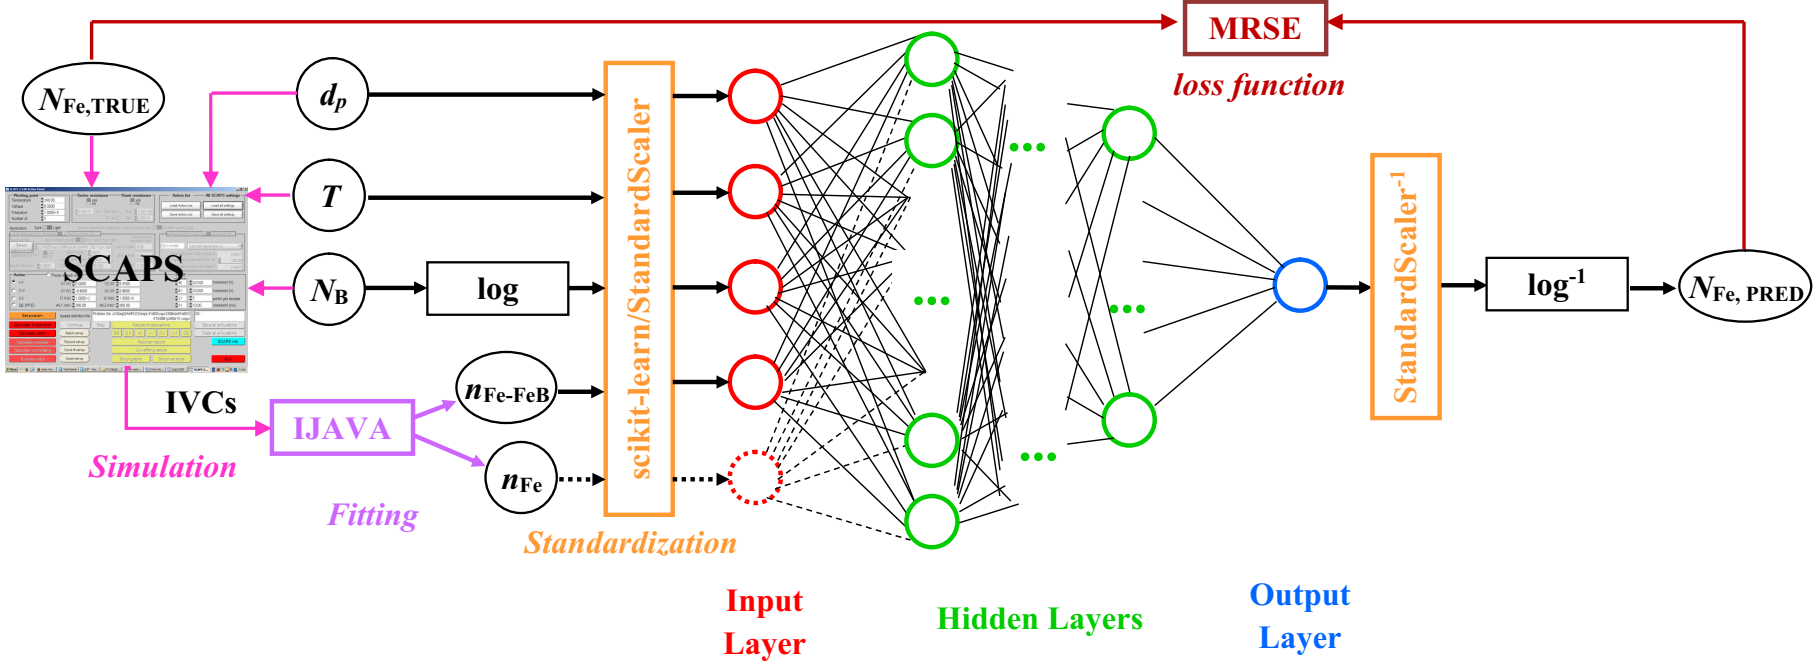
\includegraphics[width=0.9\textwidth]{Chem}
\caption{Schematic of deep learning based approach  for predicting the iron concentration.
Additional details are discussed in the body of the article.}
\label{fig_chem}
\end{figure}


\section{Simulation Details}

The calculation presented here uses simple $n^+-p$ structure shown in inset in Fig.~\ref{figIV}.
The initial thickness of each layer $d_n=0.5$~$\mu$m and $d_p=300$~$\mu$m respectively;
$n^+$ is the emitter layer with the donor concentration $N_\mathrm{D}=10^{19}$~cm$^{-3}$ and $10^{15}-10^{17}$~cm$^{-3}$ is the acceptor concentration $N_\mathrm{A}$ of the $p$ base layer,
which is uniformly doped with boron.


The simulations  were carried out over the temperature range $290-340$~K.
It should be noted that SCAPS only takes into account the simplified temperature dependencies of density of states
and  thermal  velocity of carriers.
Therefore the SCAPS setting file was created for each temperature using the material and defect parameters of Tables~\ref{tabMaterial} and \ref{tabDefect} respectively.



\begin{equation}
\label{eqEg}
    E_G(T)=E_G(0)-\alpha\Theta\left\{\frac{1-3\Delta^2}{\exp\left(\frac{\Theta}{T}\right)-1}
    +\frac{3\Delta^2}{2}\left(\sqrt[6]{1+\frac{\pi^2}{3(1+\Delta^2)}\left(\frac{2T}{\Theta}\right)^2
    +\frac{3\Delta^2-1}{4}\left(\frac{2T}{\Theta}\right)^3+\frac{8}{3}\left(\frac{2T}{\Theta}\right)^4
    +\left(\frac{2T}{\Theta}\right)^6}-1\right)\right\}\,,
\end{equation}
where
$E_G(0)=1.1701$~eV,
$\alpha=3.23\times10^{-4}$~eV/K,
$\Theta=446$~K,
$\Delta=0.51$.


\begin{equation}
\label{eqDelEg}
    \Delta E_G=4.20\times10^{-5}\left[\ln\left(\frac{N_B}{10^{14}}\right)\right]^3\,;\qquad
     \Delta E_G=4.72\times10^{-5}\left[\ln\left(\frac{N_A}{10^{14}}\right)\right]^3\,,
\end{equation}

\begin{equation}
\label{eqVth}
    \upsilon_{\mathrm{th},n}=\sqrt{\frac{8qkT}{0.28m_0\pi}}\,;\qquad
    \upsilon_{\mathrm{th},p}=\sqrt{\frac{8qkT}{0.41m_0\pi}}\,,
\end{equation}
where
$m_0$ is the free electron mass.


\begin{eqnarray}
% \nonumber to remove numbering (before each equation)
  \left(\frac{m^*_{dC}}{m_0}\right)^{1.5} &=& 1.094-1.312\times10^{-5}T+6.753\times10^{-7}T^2+4.609\times10^{-10}T^3\,, \\
  \left(\frac{m^*_{dV}}{m_0}\right)^{1.5} &=& 0.3426+3.376\times10^{-3}T-4.689\times10^{-6}T^2+2.525\times10^{-9}T^3\,.
\end{eqnarray}

\begin{eqnarray}
% \nonumber to remove numbering (before each equation)
   \nonumber C_{p} (T)&=& (7.91\times10^{-32}-4.13\times10^{-35}T+3.59\times10^{-37}T^2)\\
  &&\times\left(1+\left(564812T^{-1.6545}-1\right)\left(1-\tanh\left[\left\{\frac{p}{5\times10^{16}}\right\}^{0.29}\right]\right)\right)\,, \\
   C_{n} (T)&=& 2.8\times10^{-31}
  \times\left(1+\left(235548T^{-1.5013}-1\right)\left(1-\tanh\left[\left\{\frac{n}{5\times10^{16}}\right\}^{0.34}\right]\right)\right)\,.
\end{eqnarray}


The following recombination processes were taken into account: i) the outside surface recombination with electron and hole velocities 103 cm/s; 






The Elsevier cas-sc class is based on the
standard article class and supports almost all of the functionality of
that class. In addition, it features commands and options to format the
\begin{itemize} \item document style \item baselineskip \item front
matter \item keywords and MSC codes \item theorems, definitions and
proofs \item lables of enumerations \item citation style and labeling.
\end{itemize}

This class depends on the following packages
for its proper functioning:

\begin{enumerate}
\itemsep=0pt
\item {natbib.sty} for citation processing;
\item {geometry.sty} for margin settings;
\item {fleqn.clo} for left aligned equations;
\item {graphicx.sty} for graphics inclusion;
\item {hyperref.sty} optional packages if hyperlinking is
  required in the document;
\end{enumerate}

All the above packages are part of any
standard \LaTeX{} installation.
Therefore, the users need not be
bothered about downloading any extra packages.

\section{Installation}

The package is available at author resources page at Elsevier
(\url{http://www.elsevier.com/locate/latex}).
The class may be moved or copied to a place, usually,
\verb+$TEXMF/tex/latex/elsevier/+, %$%%%%%%%%%%%%%%%%%%%%%%%%%%%%
or a folder which will be read
by \LaTeX{} during document compilation.  The \TeX{} file
database needs updation after moving/copying class file.  Usually,
we use commands like \verb+mktexlsr+ or \verb+texhash+ depending
upon the distribution and operating system.

\section{Front matter}

The author names and affiliations could be formatted in two ways:
\begin{enumerate}[(1)]
\item Group the authors per affiliation.
\item Use footnotes to indicate the affiliations.
\end{enumerate}
See the front matter of this document for examples.
You are recommended to conform your choice to the journal you
are submitting to.

\section{Bibliography styles}

There are various bibliography styles available. You can select the
style of your choice in the preamble of this document. These styles are
Elsevier styles based on standard styles like Harvard and Vancouver.
Please use Bib\TeX\ to generate your bibliography and include DOIs
whenever available.

%Here are two sample references:
%See \citet{Fortunato2010}. Also refer \citet{Fortunato2010,NewmanGirvan2004}.
%More citations are here \citep{Fortunato2010,Vehlowetal2013}.

\section{Floats}
{Figures} may be included using the command, \verb+\includegraphics+ in
combination with or without its several options to further control
graphic. \verb+\includegraphics+ is provided by {graphic[s,x].sty}
which is part of any standard \LaTeX{} distribution.
{graphicx.sty} is loaded by default. \LaTeX{} accepts figures in
the postscript format while pdf\LaTeX{} accepts {*.pdf},
{*.mps} (metapost), {*.jpg} and {*.png} formats.
pdf\LaTeX{} does not accept graphic files in the postscript format.

%\begin{figure}
%	\centering
%		
\includegraphics[scale=.75]{figs/Fig1.pdf}
%	\caption{The evanescent light - $1S$ quadrupole coupling
%	($g_{1,l}$) scaled to the bulk exciton-photon coupling
%	($g_{1,2}$). The size parameter $kr_{0}$ is denoted as $x$ and
%	the \PMS is placed directly on the cuprous oxide sample ($\delta
%	r=0$, See also Table \protect\ref{tbl1}).}
%	\label{FIG:1}
%\end{figure}



The \verb+table+ environment is handy for marking up tabular
material. If users want to use {multirow.sty},
{array.sty}, etc., to fine control/enhance the tables, they
are welcome to load any package of their choice and
{cas-sc.cls} will work in combination with all loaded
packages.

\begin{table}[width=.9\linewidth,cols=4,pos=h]
\caption{This is a test caption. This is a test caption. This is a test
caption. This is a test caption.}\label{tbl1}
\begin{tabular*}{\tblwidth}{@{} LLLL@{} }
\toprule
Col 1 & Col 2 & Col 3 & Col4\\
\midrule
12345 & 12345 & 123 & 12345 \\
12345 & 12345 & 123 & 12345 \\
12345 & 12345 & 123 & 12345 \\
12345 & 12345 & 123 & 12345 \\
12345 & 12345 & 123 & 12345 \\
\bottomrule
\end{tabular*}
\end{table}

\section[Theorem and ...]{Theorem and theorem like environments}

{cas-sc.cls} provides a few shortcuts to format theorems and
theorem-like environments with ease. In all commands the options that
are used with the \verb+\newtheorem+ command will work exactly in the same
manner. {cas-sc.cls} provides three commands to format theorem or
theorem-like environments:

\begin{verbatim}
 \newtheorem{theorem}{Theorem}
 \newtheorem{lemma}[theorem]{Lemma}
 \newdefinition{rmk}{Remark}
 \newproof{pf}{Proof}
 \newproof{pot}{Proof of Theorem \ref{thm2}}
\end{verbatim}


The \verb+\newtheorem+ command formats a
theorem in \LaTeX's default style with italicized font, bold font
for theorem heading and theorem number at the right hand side of the
theorem heading.  It also optionally accepts an argument which
will be printed as an extra heading in parentheses.

\begin{verbatim}
  \begin{theorem}
   For system (8), consensus can be achieved with
   $\|T_{\omega z}$ ...
     \begin{eqnarray}\label{10}
     ....
     \end{eqnarray}
  \end{theorem}
\end{verbatim}

\newtheorem{theorem}{Theorem}

\begin{theorem}
For system (8), consensus can be achieved with
$\|T_{\omega z}$ ...
\begin{eqnarray}\label{10}
....
\end{eqnarray}
\end{theorem}

The \verb+\newdefinition+ command is the same in
all respects as its \verb+\newtheorem+ counterpart except that
the font shape is roman instead of italic.  Both
\verb+\newdefinition+ and \verb+\newtheorem+ commands
automatically define counters for the environments defined.

The \verb+\newproof+ command defines proof environments with
upright font shape.  No counters are defined.


\section[Enumerated ...]{Enumerated and Itemized Lists}
{cas-sc.cls} provides an extended list processing macros
which makes the usage a bit more user friendly than the default
\LaTeX{} list macros.   With an optional argument to the
\verb+\begin{enumerate}+ command, you can change the list counter
type and its attributes.

\begin{verbatim}
 \begin{enumerate}[1.]
 \item The enumerate environment starts with an optional
   argument `1.', so that the item counter will be suffixed
   by a period.
 \item You can use `a)' for alphabetical counter and '(i)' for
   roman counter.
  \begin{enumerate}[a)]
    \item Another level of list with alphabetical counter.
    \item One more item before we start another.
    \item One more item before we start another.
    \item One more item before we start another.
    \item One more item before we start another.
\end{verbatim}

Further, the enhanced list environment allows one to prefix a
string like `step' to all the item numbers.

%\pagebreak
\begin{verbatim}
 \begin{enumerate}[Step 1.]
  \item This is the first step of the example list.
  \item Obviously this is the second step.
  \item The final step to wind up this example.
 \end{enumerate}
\end{verbatim}

\section{Cross-references}
In electronic publications, articles may be internally
hyperlinked. Hyperlinks are generated from proper
cross-references in the article.  For example, the words
\textcolor{black!80}{Fig.~1} will never be more than simple text,
whereas the proper cross-reference \verb+\ref{tiger}+ may be
turned into a hyperlink to the figure itself:
\textcolor{blue}{Fig.~1}.  In the same way,
the words \textcolor{blue}{Ref.~[1]} will fail to turn into a
hyperlink; the proper cross-reference is \verb+\cite{Knuth96}+.
Cross-referencing is possible in \LaTeX{} for sections,
subsections, formulae, figures, tables, and literature
references.

\section{Bibliography}

Two bibliographic style files (\verb+*.bst+) are provided ---
{model1-num-names.bst} and {model2-names.bst} --- the first one can be
used for the numbered scheme. This can also be used for the numbered
with new options of {natbib.sty}. The second one is for the author year
scheme. When  you use model2-names.bst, the citation commands will be
like \verb+\citep+,  \verb+\citet+, \verb+\citealt+ etc. However when
you use model1-num-names.bst, you may use only \verb+\cite+ command.

\verb+thebibliography+ environment.  Each reference is a
\verb+\bibitem+ and each \verb+\bibitem+ is identified by a label,
by which it can be cited in the text:

\noindent In connection with cross-referencing and
possible future hyperlinking it is not a good idea to collect
more that one literature item in one \verb+\bibitem+.  The
so-called Harvard or author-year style of referencing is enabled
by the \LaTeX{} package {natbib}. With this package the
literature can be cited as follows:


\begin{enumerate}[\textbullet]
\item Parenthetical: \verb+\citep{WB96}+ produces (Wettig \& Brown, 1996).
\item Textual: \verb+\citet{ESG96}+ produces Elson et al. (1996).
\item An affix and part of a reference:
\verb+\citep[e.g.][Ch. 2]{Gea97}+ produces (e.g. Governato et
al., 1997, Ch. 2).
\end{enumerate}

In the numbered scheme of citation, \verb+\cite{<label>}+ is used,
since \verb+\citep+ or \verb+\citet+ has no relevance in the numbered
scheme.  {natbib} package is loaded by {cas-sc} with
\verb+numbers+ as default option.  You can change this to author-year
or harvard scheme by adding option \verb+authoryear+ in the class
loading command.  If you want to use more options of the {natbib}
package, you can do so with the \verb+\biboptions+ command.  For
details of various options of the {natbib} package, please take a
look at the {natbib} documentation, which is part of any standard
\LaTeX{} installation.

\appendix
\section{My Appendix}
Appendix sections are coded under \verb+\appendix+.

\verb+\printcredits+ command is used after appendix sections to list
author credit taxonomy contribution roles tagged using \verb+\credit+
in frontmatter.

\printcredits

\section*{Acknowledgment}

%The authors would like to thank...
This work was supported by National Research Foundation  of Ukraine
(project number 2020.02/0036)

%% Loading bibliography style file
%\bibliographystyle{elsarticle-num}
\bibliographystyle{model1-num-names}
%\bibliographystyle{cas-model2-names}

% Loading bibliography database
\bibliography{olikh}


%\vskip3pt

%\bio{}
%Author biography without author photo.
%Author biography. Author biography. Author biography.
%Author biography. Author biography. Author biography.
%Author biography. Author biography. Author biography.
%Author biography. Author biography. Author biography.
%Author biography. Author biography. Author biography.
%Author biography. Author biography. Author biography.
%Author biography. Author biography. Author biography.
%Author biography. Author biography. Author biography.
%Author biography. Author biography. Author biography.
%\endbio
%
%\bio{figs/pic1}
%Author biography with author photo.
%Author biography. Author biography. Author biography.
%Author biography. Author biography. Author biography.
%Author biography. Author biography. Author biography.
%Author biography. Author biography. Author biography.
%Author biography. Author biography. Author biography.
%Author biography. Author biography. Author biography.
%Author biography. Author biography. Author biography.
%Author biography. Author biography. Author biography.
%Author biography. Author biography. Author biography.
%\endbio
%
%\bio{figs/pic1}
%Author biography with author photo.
%Author biography. Author biography. Author biography.
%Author biography. Author biography. Author biography.
%Author biography. Author biography. Author biography.
%Author biography. Author biography. Author biography.
%\endbio


\end{document}

